\begin{figure}[H]
    \centering
    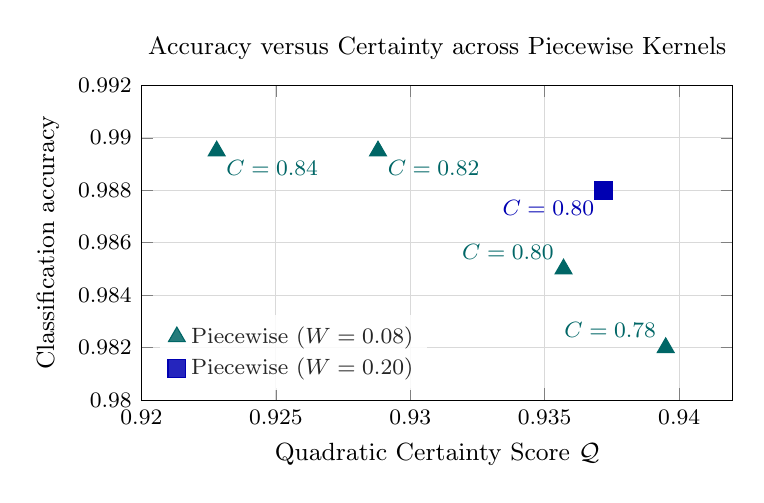
\begin{tikzpicture}
        \begin{axis}[
            width=0.75\textwidth,
            height=0.46\textwidth,
            xlabel={Quadratic Certainty Score $\mathcal Q$},
            ylabel={Classification accuracy},
            xmin=0.920, xmax=0.942,
            ymin=0.980, ymax=0.992,
            xtick={0.920, 0.925, 0.930, 0.935, 0.940},
            ytick={0.980, 0.982, 0.984, 0.986, 0.988, 0.990, 0.992},
            xticklabel style={/pgf/number format/fixed, /pgf/number format/precision=3},
            yticklabel style={/pgf/number format/fixed, /pgf/number format/precision=3},
            grid=both,
            grid style={line width=0.3pt, draw=gray!30},
            tick label style={font=\footnotesize},
            label style={font=\small},
            title style={font=\small},
            title={Accuracy versus Certainty across Piecewise Kernels},
            legend pos = south west,
            legend style={font=\footnotesize, draw=none, fill=white, fill opacity=0.85},
        ]
            % W=0.08 points
            \addplot[only marks, mark=triangle*, mark size=3.5pt, color=teal!80!black] coordinates {
                (0.9395, 0.9820)
                (0.9357, 0.9850)
                (0.9288, 0.9895)
                (0.9228, 0.9895)
            };
            \addlegendentry{Piecewise ($W=0.08$)}

            % W=0.20 point
            \addplot[only marks, mark=square*, mark size=3.2pt, color=blue!70!black] coordinates {
                (0.9372, 0.9880)
            };
            \addlegendentry{Piecewise ($W=0.20$)}

            % Annotations
            \node[anchor=north east, font=\footnotesize, color=blue!70!black] at (axis cs:0.9372, 0.9880) {$C=0.80$};
            \node[anchor=south east, font=\footnotesize, color=teal!80!black] at (axis cs:0.9357, 0.9850) {$C=0.80$};
            \node[anchor=north west, font=\footnotesize, color=teal!80!black] at (axis cs:0.9288, 0.9895) {$C=0.82$};
            \node[anchor=north west, font=\footnotesize, color=teal!80!black] at (axis cs:0.9228, 0.9895) {$C=0.84$};
            \node[anchor=south east, font=\footnotesize, color=teal!80!black] at (axis cs:0.9395, 0.9820) {$C=0.78$};
        \end{axis}
    \end{tikzpicture}
    \caption{Scatterplot of classification accuracy versus Quadratic Certainty Score $\mathcal Q$ across the custom piecewise kernel configurations on the test dataset (\hyperref[sec:piecewise_results_table]{see appendix for complete table}).}
    \label{fig:piecewise_metrics}
\end{figure}